% -*- coding: utf-8; -*-

\chapter{Plano de Ação}
\label{cha:Plano de Ação}

Para modelar o sistema, foi realizada uma validação do problema. Alunos do departamento de informática da universidade foram entrevistados afim de descobrir quais dificuldades enfrentam durante o processo de matrícula e quais são as suas preferências ao montar uma grade disciplinar. O objetivo era identificar quais características de uma grade disciplinar contribuem para a satisfação do aluno e adicionar as funcionalidades necessárias no sistema e no algoritmo.

Com o problema validado, então o projeto passou por uma etapa de pesquisa. 
Foram estudados diferentes algoritmos de recomendação em contextos semelhantes ao sistema a ser desenvolvido, afim de se projetar o algoritmo que mais se adequa às necessidades do problema validado. 
Nessa etapa, também foram analisadas as fontes de informações disponibilizadas pela universidade e como cada fonte pode ser integrada no sistema. 

Após a etapa de pesquisa, o algoritmo começou a ser desenvolvido. 
Depois de obter um algoritmo minimamente viável, foi desenvolvida a interface de planejamento para mostrar o funcionamento do algoritmo. 
Tanto o algoritmo com a interface foram desenvolvidas utilizando um modelo de desenvolvimento incremental, para que o sistema passe por etapas de desenvolvimento, teste e validação com os alunos. 

A figura \ref{fig:fluxograma-acao} exemplifica o fluxo das etapas efetuadas, desde os estudos preliminares até os testes e trabalhos futuros.

\begin{figure}[ht]
    \begin{center}
    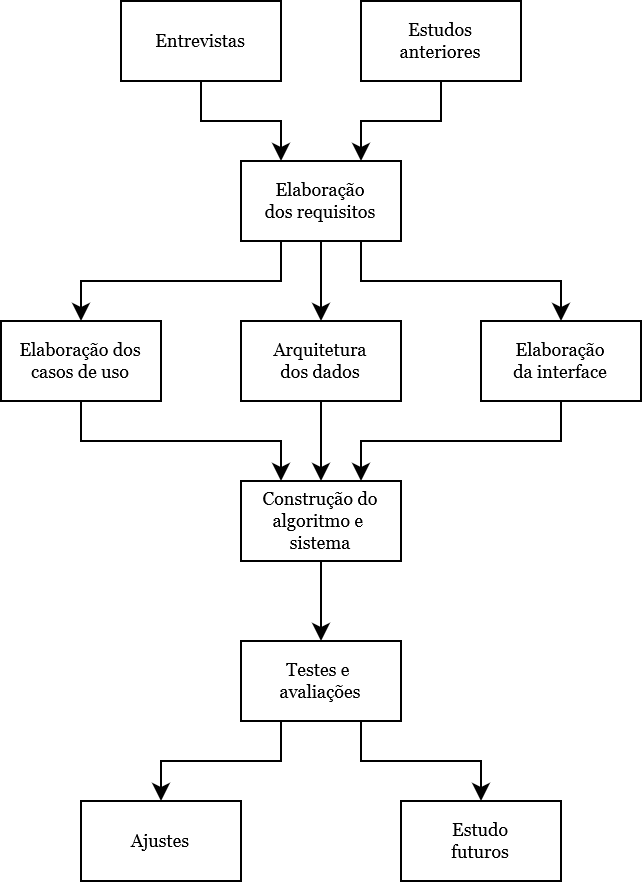
\includegraphics[width=260pt]{figuras/fluxograma-acao}
    \caption{Fluxo das etapas realizadas}
    \label{fig:fluxograma-acao}
    \end{center}
\end{figure}

\section{Cronograma original}

O cronograma inicial pode ser visualizado na figura \ref{fig:cronograma}.

\begin{figure}[ht]
    \begin{center}
    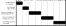
\includegraphics[width=300pt]{figuras/cronograma}
    \caption{Cronograma original do projeto}
    \label{fig:cronograma}
    \end{center}
\end{figure}

\section{Cronograma real}

O cronograma real pode ser visualizado na figura \ref{fig:cronograma-atualizado}. Surgiu uma etapa de elaboração de documentações, que dizem respeito às modelagens, diagramas e tabelas criadas antes da etapa de desenolvimento. O desenvolvimento teve seu tempo encurtado de forma extrema, mas mesmo sendo somente metade do tempo original,
foi possível implementar todas as funcionalidades planejadas.


\begin{figure}[ht]
    \begin{center}
    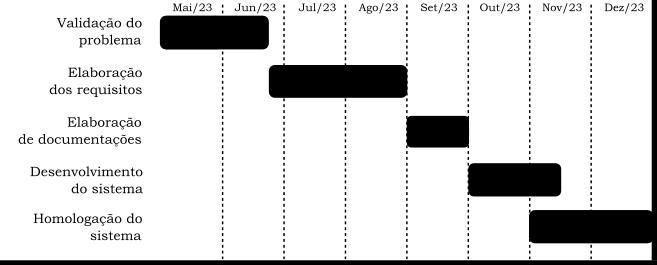
\includegraphics[width=300pt]{figuras/cronograma-atualizado}
    \caption{Cronograma atualizado do projeto}
    \label{fig:cronograma-atualizado}
    \end{center}
\end{figure}

